\section{Methodology}
\label{sec:methodology}

\subsection{Obfuscation Testing Protocol}

The core innovation of our methodology is temporal obfuscation---systematically removing temporal and contextual information while preserving structural market mechanics. The protocol involves five transformations:

\begin{enumerate}
\item Convert absolute dates (``2024-01-16'') to relative format (``Day T+0'')
\item Replace ticker symbols (``SPY'') with generic identifiers (``INDEX\_1'')
\item Remove market events (``Fed meeting'', ``earnings'')
\item Strip volatility regime context (``VIX at 14'')
\item Eliminate day-of-week patterns (``Monday'', ``OpEx Friday'')
\end{enumerate}

Preserved information includes: net gamma exposure values, directional gamma (calls vs.\ puts), spot price and flip point levels, relative time progression, and concentration metrics. Fig.~\ref{fig:obfuscation} illustrates this transformation.

\begin{figure}[!htbp]
\centering
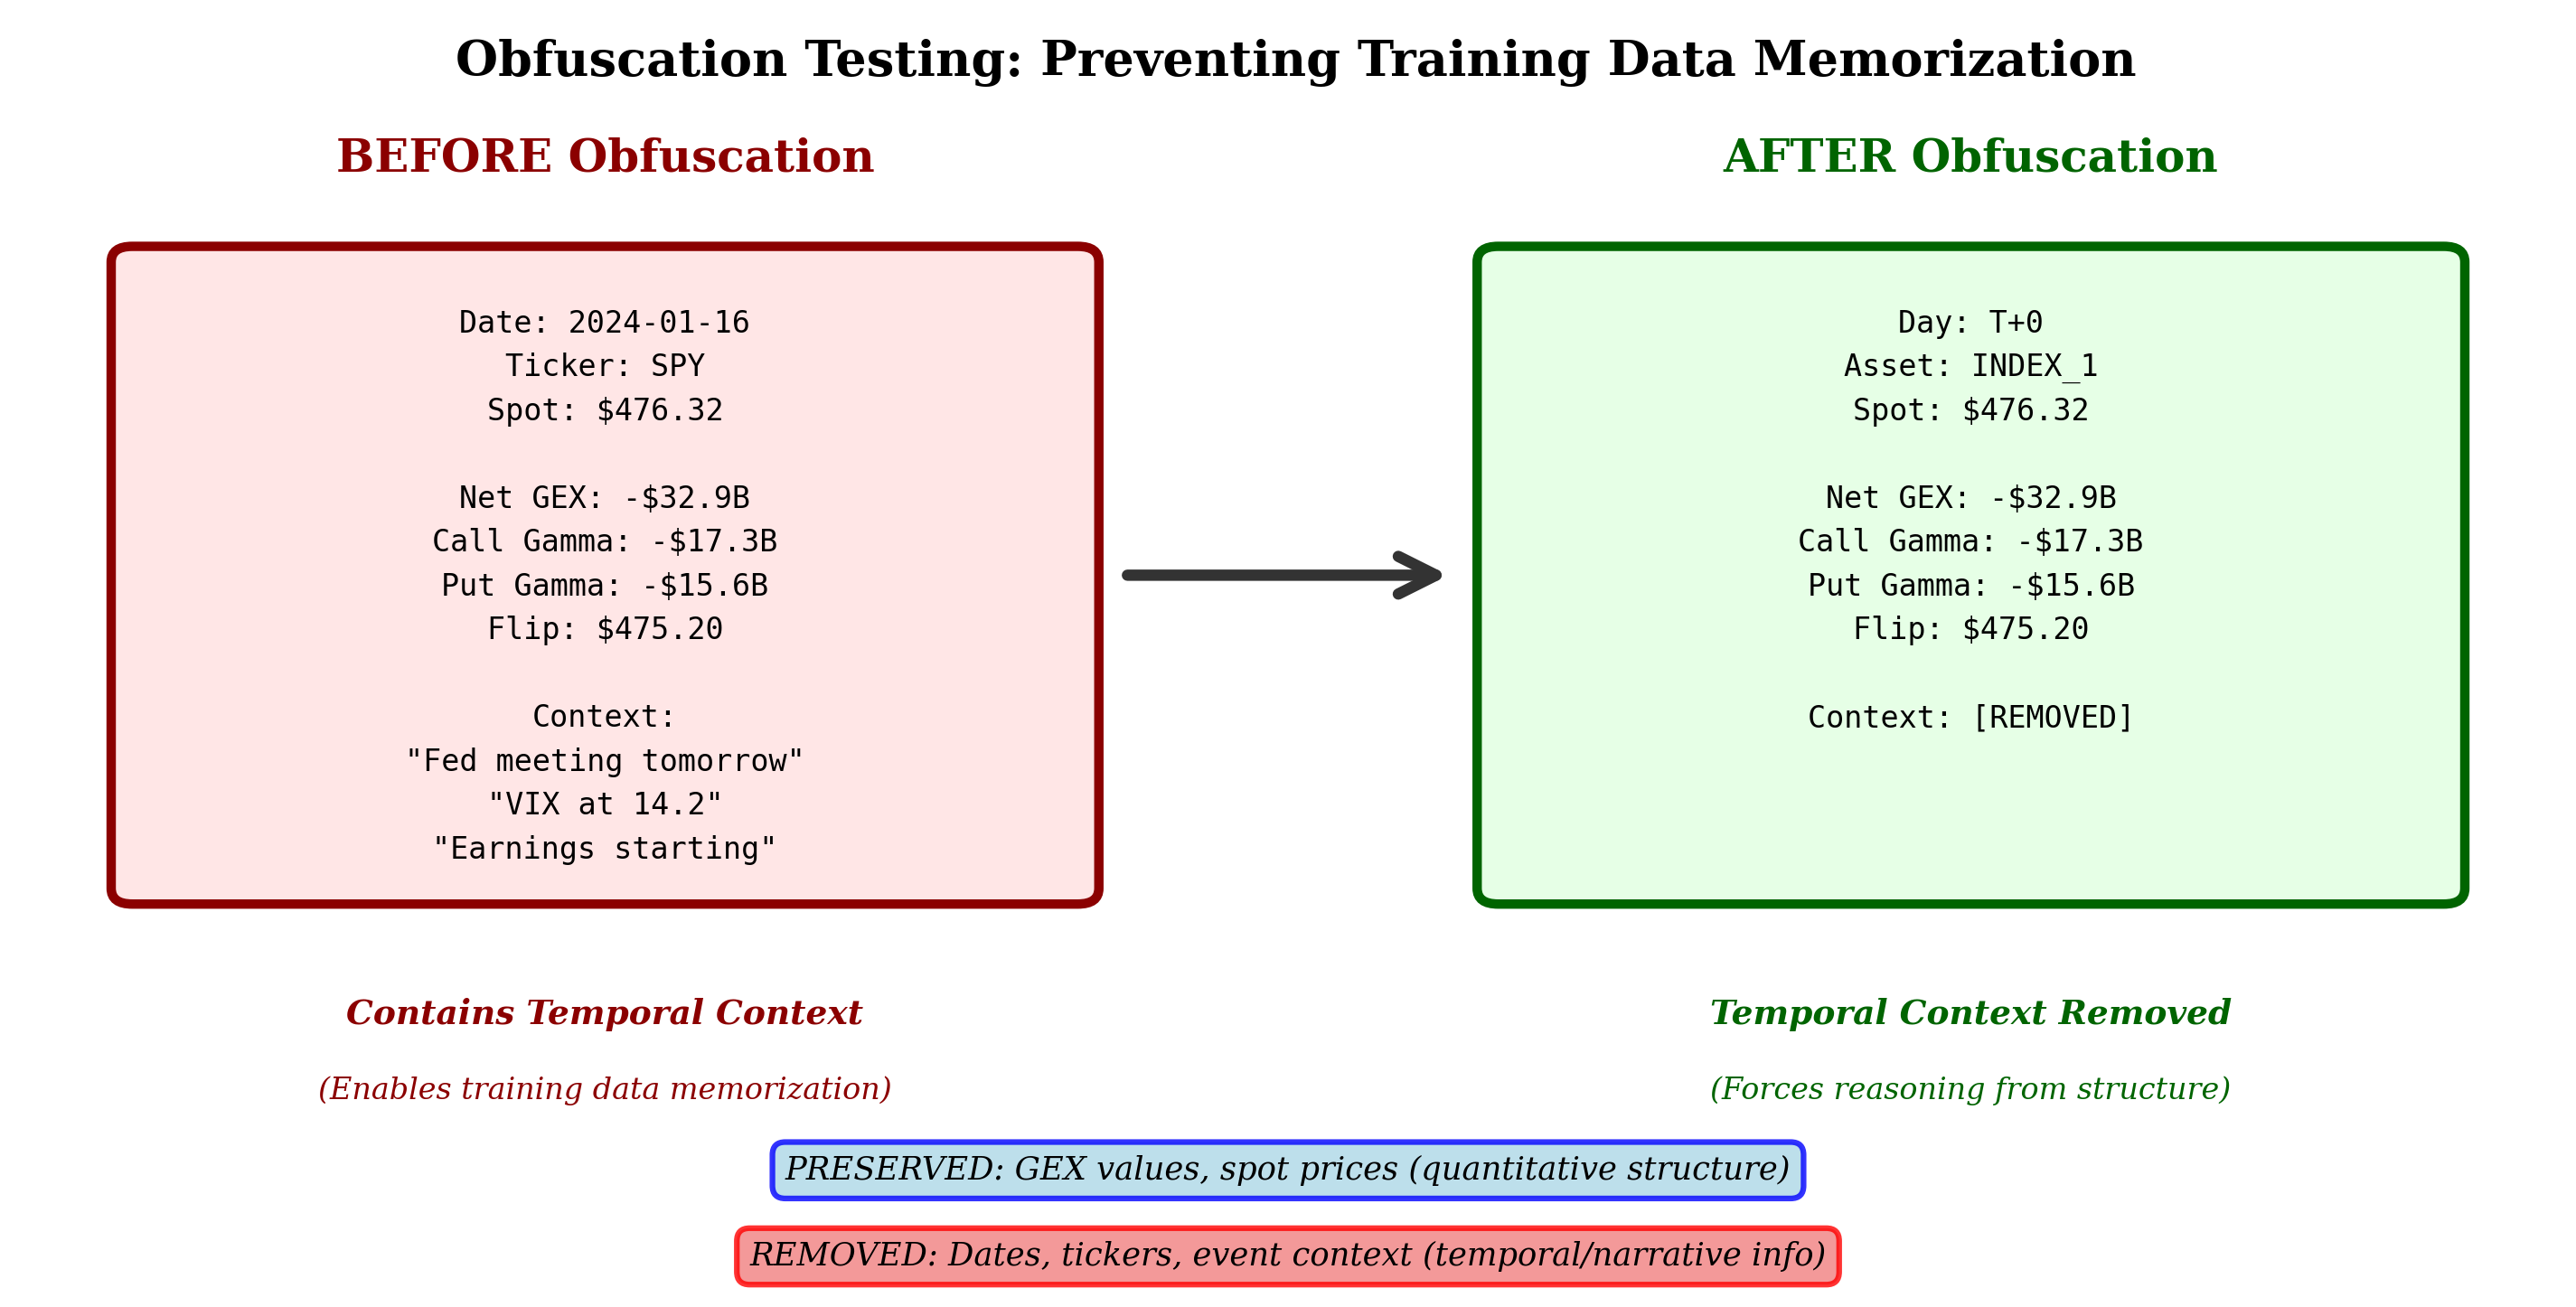
\includegraphics[width=\columnwidth]{figures/fig01_obfuscation_example.png}
\caption{Temporal obfuscation methodology. Left: Original data with dates, ticker symbols, and market context. Right: Obfuscated data preserving only structural quantitative relationships.}
\label{fig:obfuscation}
\end{figure}

This approach forces LLMs to identify patterns from quantitative relationships alone. A model memorizing ``January 2024 SPY negative gamma'' cannot succeed when presented with ``Day T+0 INDEX\_1 GEX: -\$32B''. Only genuine structural understanding enables detection under these conditions.

\subsection{Causal Framework: WHO$\rightarrow$WHOM$\rightarrow$WHAT}

Beyond detecting patterns, we require models to articulate causal mechanisms:

\textbf{WHO}: The economic actor with structural constraints (e.g., ``dealers with negative gamma exposure'').

\textbf{WHOM}: The affected market participants (e.g., ``directional traders and market makers'').

\textbf{WHAT}: The forced action and mechanism (e.g., ``must sell rallies and buy dips to maintain delta neutrality, amplifying volatility'').

This framework, derived from agent-based market microstructure theory~\cite{grossman1988liquidity,garleanu2009demand}, prevents vague pattern claims and requires specific mechanical understanding. It implements a structured form of chain-of-thought prompting~\cite{wei2022chain}, ensuring the model derives outcomes from mechanical constraints rather than recalling historical correlations.

\subsection{Single-Day Pattern Detection}
\label{subsec:single_day_method}

To ensure robustness, we test three narrative framings of the same underlying dealer constraint (Table~\ref{tab:patterns}). All reflect the same structural reality---dealers hedging option exposure---but use different conceptual lenses. Consistent detection across framings validates genuine understanding rather than keyword matching.

\begin{table}[!htbp]
\centering
\caption{Three Pattern Framings of Dealer Hedging Constraints}
\label{tab:patterns}
\small
\begin{tabular}{@{}lccc@{}}
\toprule
\textbf{Pattern} & \textbf{Framing} & \textbf{WHO} & \textbf{WHAT} \\
\midrule
Gamma Positioning & Technical/Greek & Dealers with $-\Gamma$ & Pro-cyclical hedging \\
Stock Pinning & Behavioral & Market makers & Strike convergence \\
0DTE Hedging & Temporal & Option writers & Rapid rebalancing \\
\bottomrule
\end{tabular}
\end{table}

We establish three validation levels: (1) detection rate $\geq$60\% (exceeds random chance), (2) prediction accuracy $\geq$80\% (forward returns match), and (3) correct WHO$\rightarrow$WHOM$\rightarrow$WHAT specification $\geq$90\%.

\subsection{30-Day Regime Detection Framework}

Extending from single-day patterns, we define \textit{persistent regimes} through three structural criteria applied to 30-day windows:

\textbf{Persistence}: Fraction of days sharing the dominant GEX sign.
\begin{equation}
P = \frac{\text{days with dominant sign}}{30} \geq 0.70
\end{equation}

\textbf{Magnitude}: Average absolute gamma exposure.
\begin{equation}
M = \frac{1}{30}\sum_{i=1}^{30} |\text{GEX}_i| \geq \$5\text{B}
\end{equation}

\textbf{Stability}: Maximum sign flips across 30 days.
\begin{equation}
S = \text{count}(\text{sign}(\text{GEX}_{i+1}) \neq \text{sign}(\text{GEX}_i)) \leq 5
\end{equation}

Windows meeting all three criteria are classified as persistent regimes (positive or negative); others are transitional or low-conviction. The \$5B magnitude threshold reflects dealer risk management practices, while 70\% persistence ensures directional bias significantly exceeds random binomial variation ($\approx 2.2\sigma$). Fig.~\ref{fig:regime_window} illustrates an example persistent regime.

\begin{figure}[!htbp]
\centering
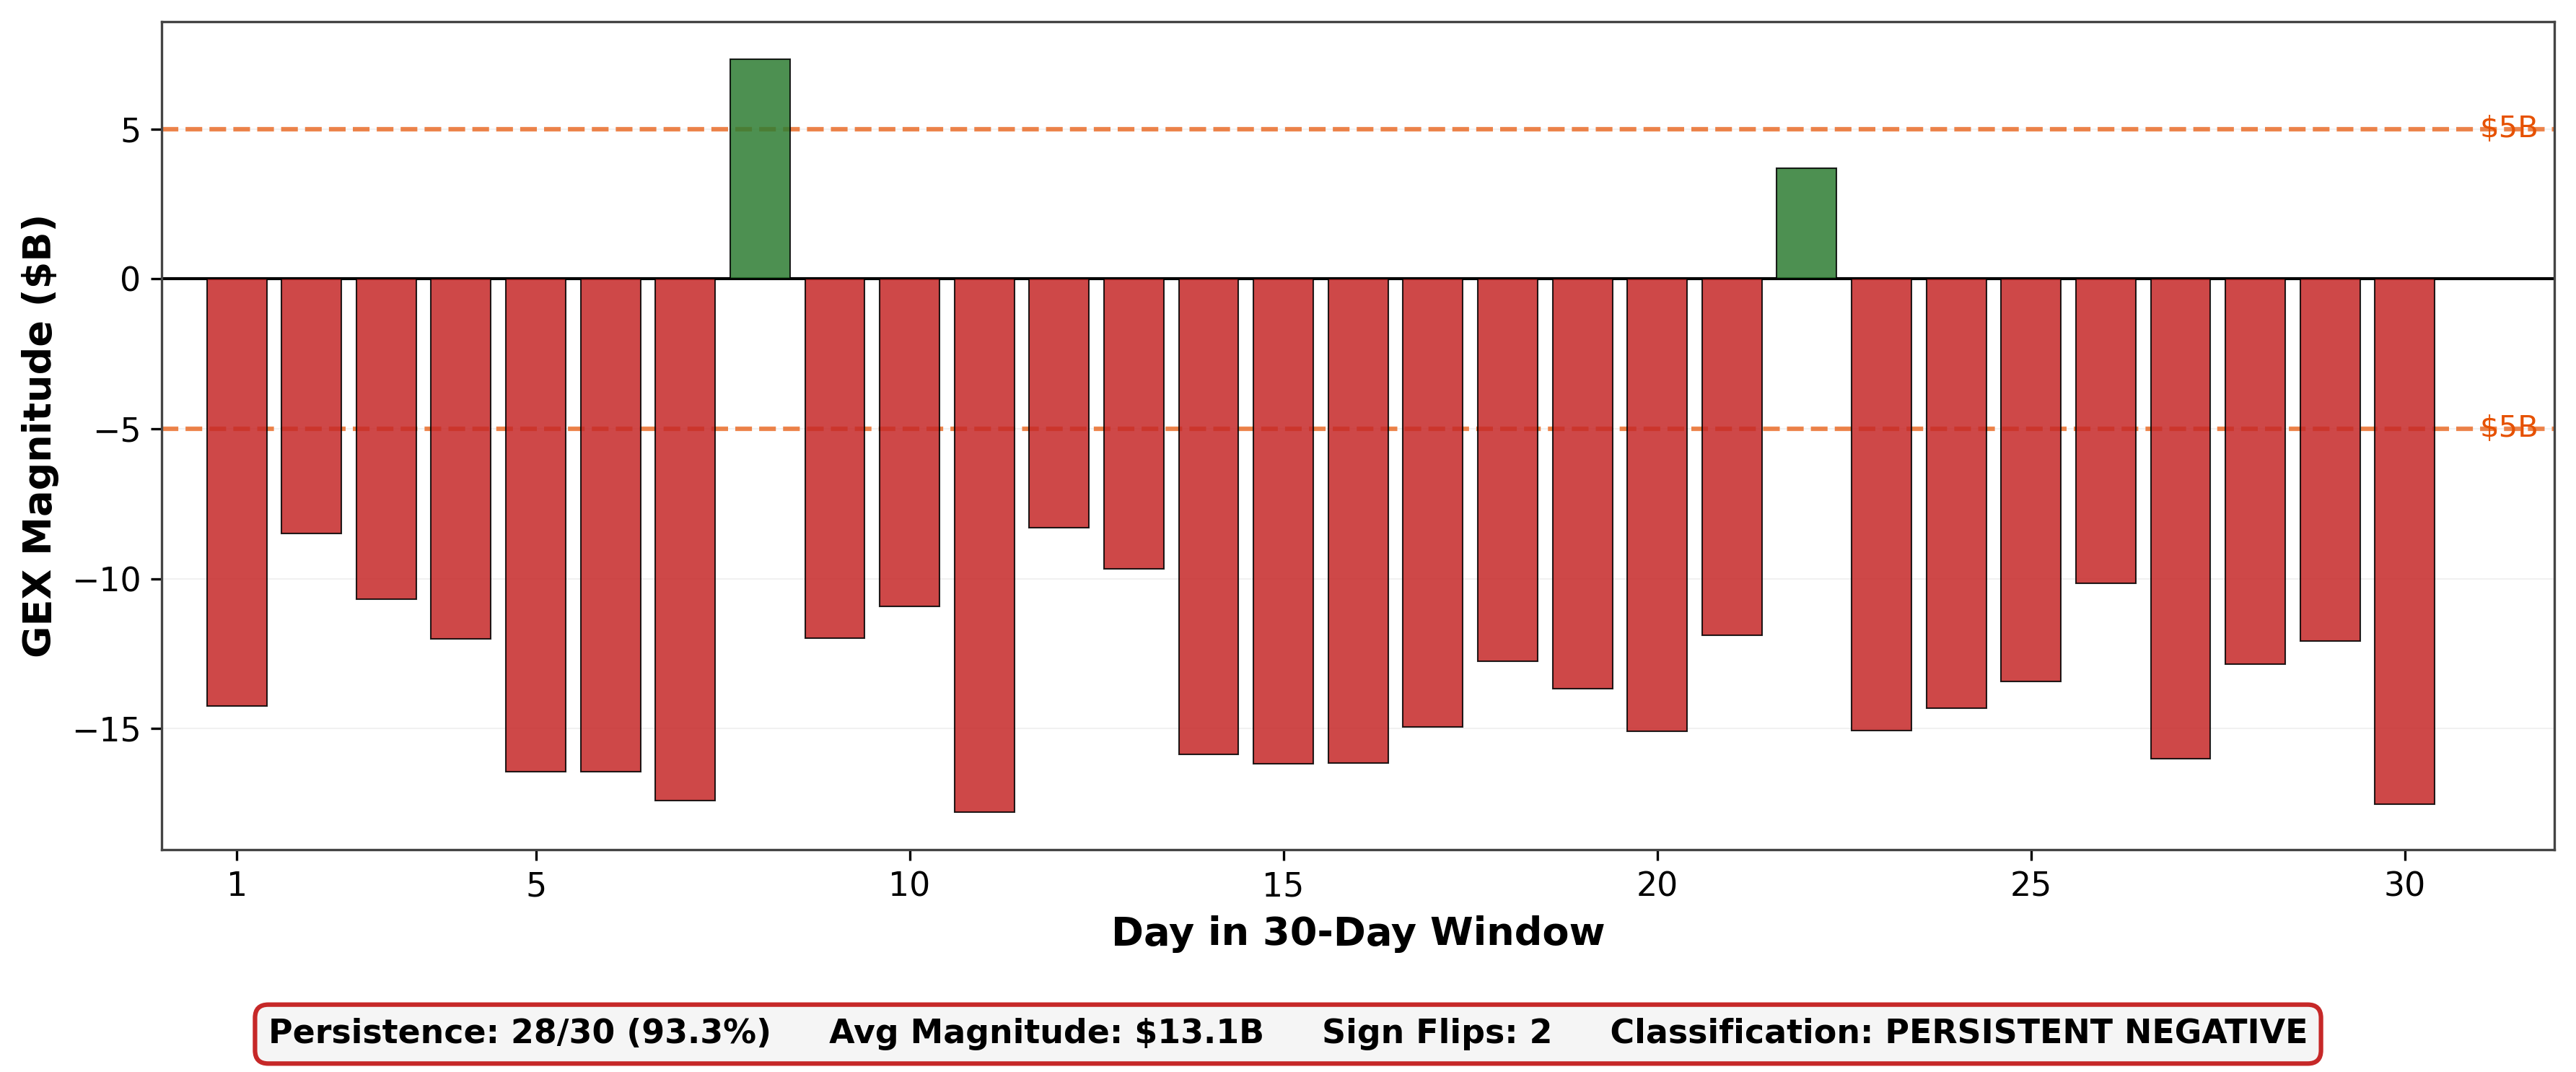
\includegraphics[width=\columnwidth]{figures/fig08_regime_window.png}
\caption{30-day persistent negative regime example. Daily GEX values showing 28/30 days negative (93.3\% persistence), average magnitude \$14.1B, and only 2 sign flips.}
\label{fig:regime_window}
\end{figure}

\subsection{GEX Calculation}

Following standard market microstructure practice~\cite{anderegg2022impact,spotgamma2021}, we calculate dealer gamma exposure from end-of-day open interest:

\begin{equation}
\text{GEX} = \sum_i \pm \text{OI}_i \times \Gamma_i \times S^2 \times 0.01 \times 100
\end{equation}

where $\Gamma_i$ is the Black-Scholes gamma at strike $i$, $\text{OI}_i$ is open interest, and $S^2$ scales gamma to dollar exposure. This open interest-based approach (GEX\_OI) measures dealer inventory positioning rather than intraday flow. While volume-based GEX may better capture 0DTE dynamics, 30-day window aggregation smooths daily measurement noise, and the underlying hedging mechanism remains constant regardless of measurement method~\cite{dim2025zero}.

We deliberately constrain analysis to gamma rather than higher-order Greeks (vanna, charm). Gamma hedging represents a universal regulatory requirement binding across institutions~\cite{mixon2009}, making it the ideal testing ground where all participants face the same fundamental constraint. Higher-order Greeks vary across proprietary implementations, precluding objective ``ground truth'' validation.

\subsection{Multi-Phase Validation Strategy}

For regime detection, we employ a five-phase protocol spanning 2020--2025:

\textbf{Phase 1} (Q1 2024 Baseline, 52 windows): Establish baseline detection rate. Success criteria: 30--50\% (demonstrates selectivity, not universal matching).

\textbf{Phase 2} (Negative Controls, 809 windows): Three synthetic tests---shuffled (404), transitional (202), and low-magnitude (203) windows. Expected: $<$10\% false positive rate.

\textbf{Phase 3} (Full 2024, 223 windows): Test Q1 generalization across all 252 trading days.

\textbf{Phase 4} (2020 Comparison, 223 windows): Test pre-0DTE era (2020, $<$5\% 0DTE volume) against post-0DTE (2024, $\approx$48\%).

\textbf{Phase 5} (Multi-Year 2020--2025, 1,412 windows): Identify when structural market shift occurred.

\subsection{Statistical Framework}

We assess performance through detection rate (fraction classified as persistent regimes), selectivity metrics (persistence gap, magnitude gap, confidence gap between detected and rejected windows), and market structure evolution ($\Delta_{\text{period}} = \text{DR}_{\text{year}_2} - \text{DR}_{\text{year}_1}$). A large positive $\Delta_{\text{period}}$ indicates fundamental market structure shift. Statistical significance uses binomial tests with Bonferroni correction.
